\documentclass[runningheads]{llncs}
\setlength{\emergencystretch}{2em}


\usepackage{url}
\usepackage{nicefrac}

% !! The following 2 lines => requires XeLaTex or LuaLaTeX
% Latin Modern fonts are an enhancement of the original Computer Modern fonts
% and are widely available in TeX distributions

\usepackage{amsmath, amssymb, mathrsfs}
\spnewtheorem{observation}[theorem]{Observation}{\bfseries}{\itshape}
\usepackage{enumitem}
\usepackage{mathtools}
\usepackage[dvipsnames]{xcolor}
\usepackage{tikz}
\usetikzlibrary{calc, patterns, patterns.meta, decorations.pathreplacing}
\usetikzlibrary{positioning,fit,arrows.meta}
\usepackage{multirow}
\usepackage{array}

\newcommand{\AC}{\mathcal{A}}
\newcommand{\BC}{\mathcal{B}}
\newcommand{\CC}{\mathcal{C}}
\newcommand{\DC}{\mathcal{D}}
\newcommand{\FC}{\mathcal{F}}
\newcommand{\GC}{\mathcal{G}}
\newcommand{\HC}{\mathcal{H}}
\newcommand{\IC}{\mathcal{I}}
\newcommand{\KC}{\mathcal{K}}
\newcommand{\NC}{\mathcal{N}}
\newcommand{\OC}{\mathcal{O}}
\newcommand{\PC}{\mathcal{P}}
\newcommand{\QC}{\mathcal{Q}}
\newcommand{\UC}{\mathcal{U}}

\newcommand{\FB}{\mathbb{F}}
\newcommand{\NB}{\mathbb{N}}
\newcommand{\QB}{\mathbb{Q}}
\newcommand{\RB}{\mathbb{R}}
\newcommand{\ZB}{\mathbb{Z}}

\newcommand{\Cbar}{\overline{C}}

%
% highlight variables
%

\usepackage{bm} % for bold‐italic math symbols
\usepackage{graphicx}

% define custom colours
\definecolor{darkblue}{RGB}{0,0,139} %  built-in dvipsnames has: DarkBlue
\definecolor{darkred}{RGB}{139,0,0} %  built-in dvipsnames has: Red4 / BrickRed / Mahogany

% newcommand: \dbx{<symbol>} → bold-italic darkblue <symbol>
\newcommand{\dbx}[1]{\textcolor{darkblue}{\bm{#1}}}
\newcommand{\drx}[1]{\textcolor{darkred}{\bm{#1}}}

\newcommand{\dbxs}[1]{\scalebox{1.1}{$\textcolor{darkblue}{\bm{#1}}$}}
\newcommand{\drxs}[1]{\scalebox{1.1}{$\textcolor{darkred}{\bm{#1}}$}}

% Define theorem styles and numbering
% 
% Define Exercises with separate numbering

% Define Examples with separate numbering

% Define proof environment (already built-in with amsthm)
% Optionally, you can customize the proof header if needed

\newcommand\restr[2]{{% we make the whole thing an ordinary symbol
  \left.\kern-\nulldelimiterspace % automatically resize the bar with \right
  #1 % the function
  \littletaller % pretend it's a little taller at normal size
  \right|_{#2} % this is the delimiter
  }}
\newcommand{\littletaller}{\mathchoice{\vphantom{\big|}}{}{}{}}

%%%%%%%%%%%%%%%%%%%%%%%%%%%%%%%%%%%%%%%%%%%%%%%%%%%%%%%%%%%%%%%%%%%%%%%%%%%


% Inner rounded boxes for each part

\newcommand{\PrivateInputs}{Private inputs}
\newcommand{\PublicInputs}{Public inputs}
\newcommand{\InCircuit}{In-circuit computations/validations}

%%%%%%%%%%%%%%%%%%%%%%%%%%%%%%%%%%%%%%%%%%%%%%%%%%%%%%%%%%%%%%%%%%%%%%%%%%%

% Merkle-root notation (avoid \root which is a TeX primitive)
\newcommand{\mroot}[1]{\mathsf{root}_{\mathtt{#1}}}

%%%%%%%%%%%%%%%%%%%%%%%%%%%%%%%%%%%%%%%%%%%%%%%%%%%%%%%%%%%%%%%%%%%%%%%%%%%

% Vectors (with and without arrow)
\newcommand{\vct}[1]{\mathbf{#1}}
% \newcommand{\vct}[1]{\vec{#1}}
% \newcommand{\vct}[1]{\vec{\mkern0mu #1}}
% \newcommand{\vct}[1]{\vec{\mkern0mu \mathbf{#1}}}
% \newcommand{\vct}[1]{\overrightarrow{\mathbf{#1}}}

% \newcommand{\vct}[1]{\overline{\vphantom{(}\mathbf{#1}}}

% \newcommand{\vct}[1]{\overline{\mathbf{#1}}}

\usepackage{calc}
\newcommand{\vcth}[1]{%
  \overline{\raisebox{0pt}[\dimexpr\height+0.8pt\relax]{$\mathbf{#1}$}}
}

\usepackage{hyperref}

% QUAL alias for the qualified set, standard DKG notation
\newcommand{\QUAL}{\mathsf{QUAL}}
\newcommand{\HK}{\mathsf{H}_{\mathsf{K}}}
\newcommand{\HP}{\mathsf{H}_{\mathsf{P}}}
\newcommand{\Nmax}{N_{\max}}
\newcommand{\Kmax}{K_{\max}}

%%%%%%%%%%%%%%%%%%%%%%%%%%%%%%%%%%%%%%%%%%%%%%%%%%%%%%%%%%%%%%%%%%%%%%%%%%%

% authblk loaded above

\title{Non-Interactive Distributed Key Generation on the EVM with Per-Application Committee Keys}
\titlerunning{Non-Interactive DKG on the EVM}
\author{Anonymous Submission}
\authorrunning{Anonymous}
\institute{}

\begin{document}
\maketitle

% Fragment: abstract, Section 1 (Introduction), Section 2 (Related Work and
% Comparison), Section 3 (Model, Goals and Notation). No preamble; assumes the
% macros of main.tex (\GC, \FB, \HK, \HP, \Kmax, \Nmax, \QUAL, \QC, \mroot).

\begin{abstract}
We present a distributed key generation protocol on a public EVM chain in which every contribution is a publicly verifiable Feldman dealing carried by a Groth16 proof and verified with one fixed-size check over eight public inputs, whatever the committee size, so no complaint phase exists. One epoch deals a pool of $\Kmax$ independent committee keys inside the same proof, and a second proof, one per epoch, finalizes it: the contract stores all $\Kmax$ keys and their share-commitment roots in one transaction. Every application claims its own pool key, so a copied ciphertext decrypts under an unrelated key, or adds an organizer key revealed once, application-wide, before which the contract admits no partial decryption. A secrecy game with corrupt organizers, submitters and $f$ committee members admits DDH reductions for both modes under stated corruption, random-oracle and proof-system assumptions; the automatic mode additionally relies on Groth16's weak simulation-extractability in the algebraic group model. At a committee bound of $32$ and a pool of $16$, the contribution circuit has $5.90$\,M constraints and proves in $3.5$\,s; a contribution costs $0.50$--$1.31$\,M gas and the finalization of all $16$ keys $2.2$--$2.8$\,M.

\keywords{Distributed key generation \and Threshold decryption \and Publicly verifiable secret sharing \and zk-SNARKs \and EVM.}
\end{abstract}

%%%%%%%%%%%%%%%%%%%%%%%%%%%%%%%%%%%%%%%%%%%%%%%%%%%%%%%%%%%%%%%%%%%%%%%%%%%%%%%%
\section{Introduction}
\label{sec:intro}

A distributed key generation protocol lets $n$ parties produce a public key whose secret is Shamir-shared so that any $t$ of them can decrypt \cite{desmedt1989threshold}, while nobody ever holds it. Pedersen-style DKGs \cite{pedersen1991threshold} let recipients check their own shares and settle faulty dealings by interactive complaints; on a public chain that dispute logic runs in a contract, at block granularity, and is itself an attack surface \cite{schindler2019ethdkg,sober2023zksnark}. Publicly verifiable secret sharing \cite{stadler1996pvss,schoenmakers1999pvss,fouque2001oneround} removes complaints in principle, but its proofs cost $\Theta(n)$ group operations per dealing, in groups the EVM does not expose or prices at hundreds of thousands of gas.

A general-purpose succinct proof changes the accounting: a Feldman dealing carried by a Groth16 proof is accepted or rejected by one fixed-size verification with eight public inputs, whatever $n$ and $t$; what grows with the committee is the calldata of commitments and encrypted shares, so a contribution transaction costs $0.50$\,M gas at $n = 4$ and $1.31$\,M at $n = 32$ in our build (\S\ref{sec:impl}). The rest of the paper makes that check bind the right data and lets one committee serve many applications under keys that do not leak into each other.

\paragraph{Motivating application.} Consider an encrypted voting service: ballots are exponential-ElGamal ciphertexts, aggregated homomorphically off chain, and only authorized tally ciphertexts are submitted for threshold decryption. The aggregate submitter does not know the summed randomness, so the proof of knowledge with which threshold ElGamal classically closes its decryption oracle \cite{shoup2002threshold} is unavailable. Elections need isolated keys; some also need an organizer-controlled, application-wide release. Ballot validity, eligibility, aggregation correctness and tally authorization lie outside this layer; the protocol alone does not stop an authorized submitter from submitting an individual ballot.

\paragraph{Contributions.}
\begin{enumerate}[leftmargin=1.5em,nosep]
  \item \emph{Succinctly verified dealings of a key pool.} Each contribution deals $\Kmax$ independent Feldman polynomials to the whole committee and is verified on chain by one fixed-size Groth16 verification with eight public inputs; an invalid dealing is refused at submission, so no dispute phase exists. One finalization proof per epoch aggregates the accepted dealings of all $\Kmax$ keys and evaluates every member's share commitments; the contract stores $\Kmax$ keys and Merkle roots in one transaction, so every key is usable the moment the epoch is live (\S\ref{sec:protocol}).
  \item \emph{Per-application keys in two modes, with a security model.} Every application claims one pool key. An \emph{automatic} application is decrypted by any $t$ members inside its decryption window; an \emph{organizer-locked} one adds an organizer key, $\mathsf{PK}_{\mathtt{aid}} = P_j + \mathsf{PK}_{\mathtt{org}}$, whose secret is revealed once, application-wide, before which honest nodes (fewer than $t$ corrupt) release no partial. A secrecy game with corrupt organizers, submitters and $f$ members yields DDH reductions for a locked application before its reveal ($n - f \ge t$, Theorem~\ref{thm:locked}) and for an automatic one ($f < t$, Theorem~\ref{thm:automatic}), with their assumptions stated (\S\ref{sec:security}).
  \item \emph{Verification devices and an implementation.} A binding random-linear-combination commitment, gated by public counts so calldata carries no padding, keeps every verifier at $7$--$15$ public inputs; we state its exact hypotheses and the forgery when one is dropped (Lemma~\ref{lem:brlc}). A canonical interpolation check gives the combine proof one accepted Lagrange vector modulo $q$ (\S\ref{sec:succinct}). Three contracts and four circuits are measured with their real verifiers on a local testbed (\S\ref{sec:impl}).
\end{enumerate}

\begin{table}[tb]
\centering
\caption{Dealing verification in DKGs with a public bulletin board. PV: publicly verifiable dealing. SRS: the scheme needs a per-circuit structured reference string; unmarked rows need no trusted setup. Size: what one dealing publishes.}
\label{tab:related}
\scriptsize
\setlength{\tabcolsep}{3pt}
\renewcommand{\arraystretch}{1.1}
\begin{tabular}{@{}>{\raggedright\arraybackslash}p{2.9cm}>{\raggedright\arraybackslash}p{1.4cm}>{\raggedright\arraybackslash}p{3.1cm}>{\raggedright\arraybackslash}p{1.6cm}>{\raggedright\arraybackslash}p{2.3cm}@{}}
\hline
Protocol & Check & Verifier per dealing & Size per dealing & Verified by \\
\hline
Pedersen; Gennaro et al.; Shutter \cite{pedersen1991threshold,gennaro1999secure,shutter2024} & complaints & $O(t)$ exp., recipient only & $O(t)$ + $n$ private & parties; synchronous rounds \\
Fouque--Stern; SCRAPE; ALBATROSS; Kate et al.\ \cite{fouque2001oneround,cascudo2017scrape,cascudo2020albatross,kate2024classgroups} & PV & $O(n)$ Paillier, group or class-group ops & $O(n)$ & anyone \\
Gurkan et al.; Groth NI-DKG \cite{gurkan2021aggregatable,groth2021nidkg} & PV & $O(n)$ exp.\ + pairings; aggregatable & $O(n)$ & anyone; BFT replicas \\
Ferveo \cite{bebel2022ferveo} & PV & $O(n)$ exp.\ + pairings & $O(n)$ & BFT validators \\
EthDKG \cite{schindler2019ethdkg} & complaints on chain & $O(t)$ exp.\ per recipient; contract adjudicates & $O(t+n)$ & EVM contract; block windows \\
Sober et al.\ \cite{sober2023zksnark} & complaints on chain & SNARK-checked rebuttal (SRS) & $O(t+n)$ & EVM contract; block windows \\
This work & PV & one Groth16 verification, $8$ public inputs (SRS) & $\Kmax(2t{+}n)$ ${+}\,5n$ words, $\Kmax$ dealings & EVM contract; block windows \\
\hline
\end{tabular}
\end{table}

%%%%%%%%%%%%%%%%%%%%%%%%%%%%%%%%%%%%%%%%%%%%%%%%%%%%%%%%%%%%%%%%%%%%%%%%%%%%%%%%
\section{Related Work and Comparison}
\label{sec:related}

Pedersen's DKG \cite{pedersen1991threshold} runs $n$ Feldman instances \cite{feldman1987practical} in parallel; Gennaro et al.\ showed that a rushing adversary biases its key \cite{gennaro1999secure} and that the biased key stays safe for discrete-log applications such as ElGamal \cite{gennaro2003applications}, the position this paper takes. Kate and Goldberg moved DKG to the Internet setting \cite{kate2009dkg}; asynchronous DKGs \cite{kokoris2020asynchronous,das2022practical,abraham2023bingo,das2023practical,zhang2023practical,abraham2025quadratic,feng2025coin} reach near-quadratic communication and adaptive security but rest on asynchronous VSS and agreement primitives \cite{bacho2025sok}, unneeded on a chain that already orders messages; SPRINT \cite{benhamouda2024sprint} targets threshold signing.

Complaint-free dealing is not new. Publicly verifiable secret sharing \cite{stadler1996pvss,schoenmakers1999pvss} and Fouque and Stern's one-round DKG \cite{fouque2001oneround} began the line; SCRAPE \cite{cascudo2017scrape} made verification linear, ALBATROSS \cite{cascudo2020albatross} batched it, Gurkan et al.\ \cite{gurkan2021aggregatable} made transcripts aggregatable, Groth's NI-DKG \cite{groth2021nidkg} uses forward-secure encryption and a bespoke proof system, Kate et al.\ \cite{kate2024classgroups} need no setup at all with class groups, and Ferveo \cite{bebel2022ferveo} deploys publicly verifiable dealings among the validators of a BFT chain, each verifier performing $\Theta(n)$ group operations per dealing.

On the EVM, EthDKG \cite{schindler2019ethdkg} ports Joint-Feldman with on-chain dispute resolution, Sober et al.\ \cite{sober2023zksnark} check the rebuttal with a zk-SNARK but keep the complaint phase, and Shutter \cite{shutter2024} runs Feldman VSS with interactive complaints in production. Table~\ref{tab:related} positions the present design: a publicly verifiable dealing, checked by the contract at a fixed verifier cost, under a per-circuit trusted setup; it separates verifier work from transcript size.

%%%%%%%%%%%%%%%%%%%%%%%%%%%%%%%%%%%%%%%%%%%%%%%%%%%%%%%%%%%%%%%%%%%%%%%%%%%%%%%%
\section{Model, Goals and Notation}
\label{sec:model}

\subsection{Notation and Primitives}
\label{subsec:prelim}

$\GC$ is a cyclic group of prime order $q$, written additively with generator $G$; DDH is assumed hard. The implementation uses BabyJubJub's prime-order subgroup (cofactor $8$) over the BN254 scalar field $\FB_p$, $p > q$, the circuits' native field, so in-circuit reduction modulo $q$ needs a bounded quotient (\S\ref{sec:succinct}). $\HK$ is Keccak-256, reduced modulo $q$ for the contract's Schnorr challenges and modulo $p$ for the calldata-binding challenges of \S\ref{sec:succinct}; $\HP$ is Poseidon \cite{grassi2021poseidon}. The contract checks points canonical, on-curve and, where meaningful, non-identity; whoever multiplies a secret into a point checks its subgroup. An epoch has $n \le \Nmax$ members, threshold $t$, $f$ corrupt, and $\Kmax$ pool keys ($\Nmax = 32$, $\Kmax = 16$); $\QUAL \subseteq [n]$, $|\QUAL| \ge m_{\min} \ge t$, are the accepted dealers, frozen at finalization; $\QC$, $|\QC| = s \ge t$, those whose partials are combined.

\paragraph{Feldman VSS \cite{shamir1979share,feldman1987practical}.} A dealer with secret $\sigma$ samples a uniform $f$ of degree below $t$ over $\FB_q$ with $f(0) = \sigma$, sends party $u$ the share $f(u)$ and publishes $C(k) := a_k G$ per coefficient; $u$ checks
\begin{equation}
    f(u)\,G \overset{?}{=} \sum_{k=0}^{t-1} u^k\, C(k).
    \label{eq:feldman}
\end{equation}

\paragraph{Hashed ElGamal for shares.} A share $s \in \FB_q$ is encrypted under a recipient key $\mathsf{pub} = xG$ as
\begin{equation}
    (R, \sigma) := \bigl(rG,\; s + \HP(\mathsf{ctx} \,\|\, r\,\mathsf{pub}) \bmod q\bigr), \qquad r \leftarrow \FB_q,
    \label{eq:hashed-elgamal}
\end{equation}
and recovered as $s = \sigma - \HP(\mathsf{ctx} \,\|\, xR)$; $\mathsf{ctx}$ binds epoch, dealer, recipient and key index, so one ECDH value per recipient yields $\Kmax$ distinct masks; IND-CPA holds under DDH with $\HP$ a random oracle \cite{abdalla_bellare_rogaway_dhies_2001,cash_kiltz_shoup_twin_dh_2008}, a heuristic since the same $\HP$ is arithmetised in the dealing circuit (\S\ref{sec:security}, (c)). Applications use exponential ElGamal (\S\ref{sec:protocol}).

\subsection{Chain, Parties and Adversary}
\label{subsec:model}

\paragraph{Chain and parties.} We assume finality below the parties' confirmation depth, bounded inclusion of funded honest parties' transactions (phase windows are sized accordingly) and availability of accepted calldata. Registered operators form each epoch's committee by snapshot-based eligibility filtering from a block-hash seed (\S\ref{sec:protocol}), exposed to proposer bias and inclusion races: every result is conditioned on the selected committee meeting the corruption bound. Organizers register applications and submitters post ciphertexts; registry admission is a deployment assumption.

\paragraph{Adversary.} Corruptions are static \cite{canetti1999adaptive}: $f$ members and any number of other operators, organizers and submitters; honest members keep shares for the epoch's decryption horizon. The corruption bounds and cryptographic assumptions are exactly (a)--(f) of \S\ref{sec:security}, which also states which result uses which. Adaptive or proactive corruption, UC composition and setup compromise are out of scope.

\subsection{Goals}
\label{subsec:goals}

\emph{Correctness}: for a key $j$ of a live epoch, $A_j := \sum_{\ell \in \QUAL} f_\ell^{(j)}$, the stored key is $A_j(0)\,G$, the Merkle leaves $A_j(i)\,G$, honest member $i$'s share $A_j(i)$, and a combined plaintext of a well-formed ciphertext $\log_G(C_2 - \mathsf{sk}_{\mathtt{aid}} C_1)$ within the search bound. \emph{Availability}: an epoch with $m_{\min}$ accepted contributions goes live, by one finalization proof, with every key usable; a well-formed ciphertext whose gate is open is decrypted whenever $t$ honest holders are available and included. \emph{Secrecy}: the game of \S\ref{sec:security}; Table~\ref{tab:threat} states what holds under which corruption.

\begin{table}[tb]
\centering
\caption{Guarantees by adversary. Outsiders: other organizers and submitters. Gated: honest members post no partial before the application's window opens and, if locked, before its reveal. Rows 1 and 2 also need one honest accepted dealer.}
\label{tab:threat}
\scriptsize
\setlength{\tabcolsep}{3pt}
\renewcommand{\arraystretch}{1.1}
\begin{tabular}{@{}>{\raggedright\arraybackslash}p{3.3cm}>{\raggedright\arraybackslash}p{1.2cm}>{\raggedright\arraybackslash}p{7.25cm}@{}}
\hline
Adversary controls & Bound & What holds \\
\hline
Outsiders; $f$ members & $f < t$, $n - f \ge t$ & Honest application confidential while gated (Theorem~\ref{thm:automatic}) \\
Own organizer (correctly generated secret, unrevealed); $f$ members & $f < t$, $n - f \ge t$ & No leak via other applications; own one gated (Theorem~\ref{thm:locked}) \\
Outsiders; $f$ members & any $f$ & Locked application confidential until reveal (Theorem~\ref{thm:locked}) \\
$t$ members & --- & Automatic mode broken; locked keeps its organizer factor \\
Organizer and $t$ members & --- & No embargo in either mode; coalition decrypts off chain \\
Authorized submitter & any & Chooses what enters; nothing is claimed about its inputs \\
\hline
\end{tabular}
\end{table}

\section{Protocol and Design Rationale}
\label{sec:protocol}

The protocol runs in \emph{epochs}. An epoch $\mathtt{eid}$ deals a pool of $\Kmax$ independent keys $P_0, \dots, P_{\Kmax-1}$; each application registered against it claims one key. Operators hold registered share-encryption keys $\mathsf{pub}_i$ (\S\ref{sec:impl}); admission is a deployment concern. On the block axis an epoch passes a selection window, a contribution window and a key-assembly gap, then stays $\textsc{Live}$ with all $\Kmax$ keys stored.

\subsection{Committee Selection}
\label{subsec:lottery}

The initiator submits $(t, n, m_{\min}, \alpha)$ (threshold, committee size, minimum accepted contributions, oversubscription) and the contract snapshots the number $N$ of active operators, pins a seed block $b_s$ a few blocks ahead and stores $\tau := \lfloor 2^{256} \alpha n / N \rfloor$. The first claim after $b_s$ freezes $\mathsf{seed} := \mathsf{blockhash}(b_s)$; operator $\mathsf{op}$ is admissible iff $\mathsf{keccak}(\mathsf{seed} \,\|\, \mathsf{op}) < \tau$, and the first $n$ admissible claimants take the slots; only operators active before creation may claim. This is snapshot-based \emph{eligibility filtering}, not an unbiasable sampler: the seed's proposer can resample or withhold it, and inclusion latency decides among admissible claimants; \S\ref{sec:security} assumes the selected committee meets the corruption bound.

Epochs are created permissionlessly once $\mathsf{EPOCH\_DURATION}$ blocks have elapsed, or earlier once the newest epoch is $\textsc{Live}$ with at most one unclaimed key or aborted; deployment immutables floor $t$ and $n$ and cap $\alpha$, which a creation-race winner can pin every epoch to. Robustness depends on the chosen epoch's $n - t$: the floors enforce no margin, since $t = n$ is admissible, so tolerating $r$ unavailable members needs $t \le n - r$.

\subsection{Epoch Key Generation}
\label{subsec:epoch}

\paragraph{Contribution.} Each member $i$ samples, for every key $j$, $0 \le j < \Kmax$, a uniform polynomial $f_i^{(j)}(x) := \sum_{k<t} a_{i,j,k}\, x^k$ over $\FB_q$ and one nonce $r_{i,u}$ per recipient $u$, and publishes in one transaction the commitments $C_i^{(j)}(k) := a_{i,j,k}\, G$ and, for every $(j, u)$, the encrypted share
\[
    E_i^{(j)}(u) := \big(R_i(u), \sigma_i^{(j)}(u)\big)
    = \big(r_{i,u} G,\ f_i^{(j)}(u) + \HP(\mathsf{ctx}_{i,u} \| j \| r_{i,u} \mathsf{pub}_u) \bmod q\big)
\]
and a proof $\pi_i$ that \eqref{eq:feldman} holds and every $E_i^{(j)}(u)$ encrypts $f_i^{(j)}(u)$ (\S\ref{sec:succinct}). The commitments are digested per key, and the $\Kmax$ digests again into a single $\mathtt{commitmentsHash}$, which the contract stores after verifying $\pi_i$; the shares stay in calldata, whose $\Kmax(2t+n) + 5n$ words are sized by the epoch's $(t, n)$, not by the circuit's capacity (\S\ref{subsec:compact}). By Lemma~\ref{lem:dealing} an accepted contribution is a correct dealing to all $n$ recipients, so no complaint phase \cite{pedersen1991threshold,gennaro1999secure} is needed.

\paragraph{Finalization.} Let $A_j := \sum_{\ell \in \QUAL} f_\ell^{(j)}$, $\Cbar^{(j)}(k) := \sum_{\ell \in \QUAL} C_\ell^{(j)}(k)$, $P_j := \Cbar^{(j)}(0) = A_j(0)\,G$ and $D_{j,i} := \sum_{k<t} i^k\, \Cbar^{(j)}(k) = A_j(i)\,G$ for $i \in [n]$. After the contribution window, with at least $m_{\min}$ accepted contributions and the key-assembly gap elapsed, anyone may call $\mathsf{finalizeEpoch}$, with no deadline, carrying one proof for the whole pool: that the $\Cbar^{(j)}(k)$ aggregate the commitments of the transcript's dealer rows for every key $j$ and that the $D_{j,i}$ are the evaluations at every committee position (\S\ref{sec:succinct}). The rows are not the finalizer's choice: the contract requires them to be exactly the accepted set it recorded---$|\QUAL|$ distinct indices in $[n]$, each an accepted contributor with its stored $\mathtt{commitmentsHash}$, every inactive row zero---so $\QUAL$ is determined by the contract, never by a prover picking a subset. In one transaction the contract freezes $\QUAL$, stores every $P_j$ and $\mroot{j}$, a Keccak Merkle root over $\Nmax$ tagged leaves $\mathsf{keccak}(\mathtt{0x00} \,\|\, D_{j,i})$, $i \le n$, a constant empty leaf beyond $n$ and inner nodes $\mathsf{keccak}(\mathtt{0x01} \,\|\, l \,\|\, r)$, and marks the epoch $\textsc{Live}$; there is no per-key activation step. Our test deployment uses a $100$-block selection window, a $150$-block contribution window, a $10$-block gap and a $7\,200$-block epoch cadence; members attempt finalization in seed-derived stagger slots, so normally one node proves and a later one finds the epoch live. An epoch short of its committee or its $m_{\min}$ rows is dead. Every member $i \in [n]$ obtains $e_{j,i} := A_j(i)$ by decrypting the calldata, whether or not it dealt: decryption tolerates $n - t$ absent members.

\subsection{Applications and Their Keys}
\label{subsec:apps}

Registration against a $\textsc{Live}$ epoch names a non-zero field element $\mathtt{aid}$ and a policy, and claims the next unclaimed key $P_j$; every key of a live epoch is usable, so it fails only once the pool is exhausted. In the \emph{organizer-locked} mode the registrant, the organizer, also submits $\mathsf{PK}_{\mathtt{org}} = \mathsf{sk}_{\mathtt{org}} G$ with a Schnorr proof of possession $(A, z) = (wG,\ w + c\,\mathsf{sk}_{\mathtt{org}})$, where $c := \HK(\mathsf{dom}_{\mathtt{org}} \| \mathtt{eid} \| \mathtt{aid} \|\allowbreak \mathsf{PK}_{\mathtt{org}} \| A)$, checked as $zG = A + c\,\mathsf{PK}_{\mathtt{org}}$; it excludes rogue keys such as $-P_j$. The application key is $\mathsf{PK}_{\mathtt{aid}} := P_j + \mathsf{PK}_{\mathtt{org}}$. In the \emph{automatic} mode there is no organizer key: the contract records the identity and $0$, $\mathsf{PK}_{\mathtt{aid}} := P_j$, and any $t$ share holders decrypt.

A user encrypts $m$ as $(C_1, C_2) := (rG,\; mG + r\,\mathsf{PK}_{\mathtt{aid}})$, $r \leftarrow \FB_q$: exponential ElGamal, additively homomorphic, $m$ being recovered from $mG$ by a bounded search. Since every key is dealt by independent polynomials, the committee's term $A_j(0)\,C_1$ is useless under any other application's key (Theorems~\ref{thm:automatic} and~\ref{thm:locked}).

\paragraph{Policy.} Registration fixes who may submit (anyone, an allow-list or the registrant), a submission block window and a decryption window. Ciphertexts are accepted only inside the submission window and before decryption closes; partials and combines only inside the decryption window and, for a locked application, after the reveal. Honest nodes (fewer than $t$ corrupt) release no partial before this gate opens (\S\ref{sec:limits}).

\subsection{Threshold Decryption}
\label{subsec:decryption}

% Decryption of one ciphertext: submit, optional reveal (locked applications only),
% threshold partials, combine. Every arrow into the contract is a transaction.
\begin{figure}[t]
\centering
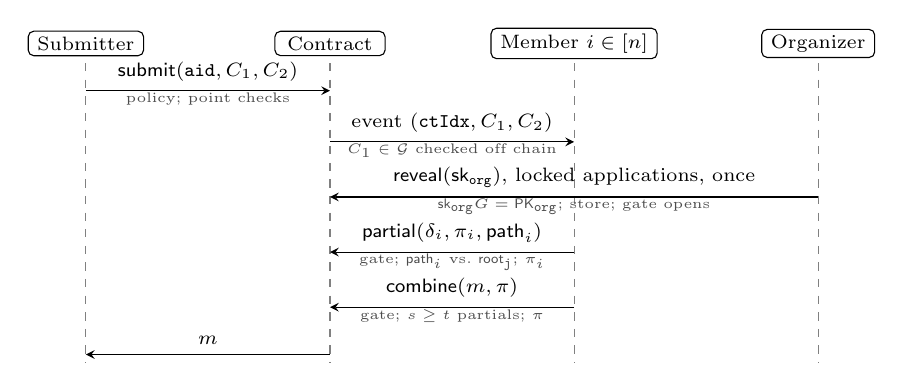
\begin{tikzpicture}[font=\scriptsize, >=stealth, note/.style={inner sep=0.5pt, font=\tiny, text=black!70}]
  \def\colS{0} \def\colC{3.1} \def\colM{6.2} \def\colO{9.3}
  \foreach \x/\n in {\colS/Submitter, \colC/Contract, \colM/Member $i \in [n]$, \colO/Organizer} {
    \node[draw, rounded corners=2pt, minimum width=1.4cm, inner ysep=2pt] at (\x,0) {\n};
    \draw[dashed, gray] (\x,-0.25) -- (\x,-4.05);
  }
  \draw[->] (\colS,-0.6) -- node[above] {$\mathsf{submit}(\mathtt{aid}, C_1, C_2)$}
    node[below, note] {policy; point checks} (\colC,-0.6);
  \draw[->] (\colC,-1.25) -- node[above] {event $(\mathtt{ctIdx}, C_1, C_2)$}
    node[below, note] {$C_1 \in \GC$ checked off chain} (\colM,-1.25);
  \draw[->] (\colO,-1.95) -- node[above] {$\mathsf{reveal}(\mathsf{sk}_{\mathtt{org}})$, locked applications, once}
    node[below, note] {$\mathsf{sk}_{\mathtt{org}} G = \mathsf{PK}_{\mathtt{org}}$; store; gate opens} (\colC,-1.95);
  \draw[->] (\colM,-2.65) -- node[above] {$\mathsf{partial}(\delta_i, \pi_i, \mathsf{path}_i)$}
    node[below, note] {gate; $\mathsf{path}_i$ vs.\ $\mroot{j}$; $\pi_i$} (\colC,-2.65);
  \draw[->] (\colM,-3.35) -- node[above] {$\mathsf{combine}(m, \pi)$}
    node[below, note] {gate; $s \ge t$ partials; $\pi$} (\colC,-3.35);
  \draw[->] (\colC,-3.95) -- node[above] {$m$} (\colS,-3.95);
\end{tikzpicture}
\caption{Decryption of a ciphertext on pool key $P_j$; arrows into the contract are transactions. Partials and the combine carry Groth16 proofs, partials also a Merkle path for $D_{j,i}$; the gate is the decryption window plus, for locked applications, the one-shot reveal.}
\label{fig:decryption}
\end{figure}


\paragraph{Submission.} $\mathsf{submitCiphertext}(\mathtt{aid}, C_1, C_2)$ carries no proof (Figure~\ref{fig:decryption}): the contract enforces the policy, assigns $\mathtt{ctIdx}$ on chain and checks both points well formed and not the identity, leaving the prime-order check to the member about to multiply its share into $C_1$, since a cofactor component would leak $e_{j,i} \bmod 8$ through its partial.

\paragraph{Partial decryption.} Any member $i \in [n]$ publishes $\delta_i := e_{j,i} C_1$ with a DLEQ proof \cite{chaum1992wallet} $(A_i, B_i, z_i) := (w_i G,\ w_i C_1,\ w_i + c_i\, e_{j,i})$, $w_i \leftarrow \FB_q$, with challenge $c_i := \HP(\mathsf{dom} \| \mathtt{eid} \| \mathtt{aid} \| \mathtt{ctIdx} \| i \|\allowbreak D_{j,i} \| C_1 \| \delta_i \| A_i \| B_i)$, verified as $z_i G = A_i + c_i D_{j,i}$ and $z_i C_1 = B_i + c_i\,\delta_i$ inside a Groth16 proof $\psi_i$ (\S\ref{sec:succinct}), and a Merkle path for $D_{j,i}$ that the contract checks against $\mroot{j}$ at leaf $i - 1$.

\paragraph{Reveal.} A locked application's organizer publishes $\mathsf{sk}_{\mathtt{org}}$ through the permissionless, one-shot $\mathsf{revealOrganizerSecret}$ call; the contract checks $\mathsf{sk}_{\mathtt{org}} G = \mathsf{PK}_{\mathtt{org}}$ and stores it. Until then no partial or combine of the application exists on chain; afterwards every past and future ciphertext is eligible, so the organizer decides \emph{when}, not \emph{which} (\S\ref{sec:limits}).

\paragraph{Combine.} Once $s \ge t$ partials from $\QC = \{x_1, \dots, x_s\}$ are on chain and the gate is open, anyone submits a proof establishing, with the canonical Lagrange coefficients $\lambda_k$ of $\QC$ (\S\ref{sec:succinct}),
\begin{align}
    \sum_{k} \lambda_k\, \delta_{x_k} = A_j(0)\, C_1, \qquad
    M = C_2 - \sum_k \lambda_k\, \delta_{x_k} - \mathsf{sk}_{\mathtt{org}}\, C_1 = mG,
    \label{eq:combine}
\end{align}
and, from the private witness $\mathsf{sk}_{\mathtt{org}}$, that $\mathsf{sk}_{\mathtt{org}} G$ is the $\mathsf{PK}_{\mathtt{org}}$ on record, trivially for an automatic application. The combiner recovers $m$ off chain by baby-step giant-step \cite{shanks1971class} (\S\ref{sec:impl}).

\paragraph{Design rationale.} Clients already produce exponential ElGamal ciphertexts and homomorphic aggregates, the organizer runs no prover, and the DKG verifies nothing application-specific. A proof of knowledge of $r$ with $C_1 = rG$ \cite{shoup2002threshold} is unavailable, since an aggregate's submitter does not know $\sum_k r_k$; the committee therefore answers any $C_1$ under any key it serves, so separation cannot come from a public additive offset ($\mathsf{PK}_{\mathtt{ep}} + \HK(\mathtt{aid})\,G$ \cite{bip32} is removed by shifting $C_2$ by $\HK(\mathtt{aid})\,C_1$) but only from independently dealt keys, pooled at one transaction and proof per member plus one finalization proof per epoch.

%%%%%%%%%%%%%%%%%%%%%%%%%%%%%%%%%%%%%%%%%%%%%%%%%%%%%%%%%%%%%%%%%%%%%%%%%%%%%%%%
\providecommand{\Rel}[1]{\mathcal{R}_{\mathsf{#1}}}
\section{Succinct Verification}
\label{sec:succinct}
\label{subsec:relations}

Recurring operations are proven in Groth16 circuits \cite{groth16} over BN254 with BabyJubJub embedded and Poseidon \cite{grassi2021poseidon} as hash. Circuits have fixed capacity $\Nmax = 32$, $\Kmax = 16$ (inactive slots masked to constants), check points on the curve, range-check the scalars marked $\in[0,q)$ below and use hint-free variable-base multiplication \cite{hisil2008twisted}. Contribution $\Rel{deal}$ has public inputs $(\mathtt{eid}, t, n, i, h_C, h_E, \rho, \beta)$; finalization $\Rel{fin}$ has $(\mathtt{eid}, t, n, a, d, \rho, \beta)$, $a = |\QUAL|$, with the transcript digest $d$ at index $4$ of $7$; partial decryption $\Rel{part}$ has the $15$ scalars $(\mathtt{eid}, \mathtt{aid}, \mathtt{ctIdx}, i, C_1, D_{j,i}, \delta_i, A_i, B_i, z_i)$, $c_i$ as in \S\ref{sec:protocol}; combine $\Rel{comb}$ has $(\mathtt{eid}, \mathtt{aid}, \mathtt{ctIdx}, t, s, h, m, \rho, \beta)$, $s = |\QC|$. Indices range over keys $j \in \{0, \dots, \Kmax-1\}$, $u, i \in [n]$, dealer rows $\ell < a$, $k < t$ ($k \le s$ in $\Rel{comb}$); all else is witness, $\vct{w}$ the transcript committed by $\beta = \mathsf{BRLC}_\rho(\vct{w})$ and $h_C\,\|\,h_E$, $d$, $h$ its Poseidon digests (\S\ref{subsec:brlc}); $g_{\ell,j} := \HP(\vct{C}_\ell^{(j)})$ digests one dealer's key-$j$ commitments:
{\small\setlength{\jot}{1pt}
\begin{align*}
\Rel{deal}:\ & a_{i,j,k}\in[0,q),\ \ C_i^{(j)}(k)=a_{i,j,k}\,G,\ \ R_i(u)=r_{i,u}\,G,\ \ S_{i,u}=r_{i,u}\,\mathsf{pub}_u,\\
& s_i^{(j)}(u)\in[0,q),\ \ s_i^{(j)}(u)\,G=\textstyle\sum_{k<t}u^k\,C_i^{(j)}(k),\ \ h_E=\HP(\vct{u}\,\|\,\vct{pub}\,\|\,\vct{E}_i),\\
& \sigma_i^{(j)}(u)=s_i^{(j)}(u)+\HP(\mathsf{ctx}_{i,u}\,\|\,j\,\|\,S_{i,u}) \bmod q,\ \ \vct{w}=\vct{C}_i\,\|\,\vct{u}\,\|\,\vct{pub}\,\|\,\vct{E}_i,\\
& h_C=\HP\big(\mathtt{eid},i,t,g_{i,0},\dots,g_{i,\Kmax-1}\big);\\
\Rel{fin}:\ & t\le a\le n\le\Nmax,\ \ \{(I_\ell,h_{C,\ell})\}_{\ell<a}=\text{frozen accepted set, contract-checked},\\
& h_{C,\ell}=\HP\big(\mathtt{eid},I_\ell,t,g_{\ell,0},\dots,g_{\ell,\Kmax-1}\big),\ \ \Cbar^{(j)}(k)=\textstyle\sum_{\ell<a}C_\ell^{(j)}(k),\\
& P_j=\Cbar^{(j)}(0),\ \ D_{j,i}=\textstyle\sum_{k<t}i^k\,\Cbar^{(j)}(k),\ \ \vct{w}=\vct{I}\,\|\,\vct{h}_C\,\|\,(P_j\,\|\,\vct{D}_j)_{j<\Kmax},\\
& \theta_j=\HP(1,j,P_j,\vct{D}_j),\ \ d=\HP\big(2,\mathtt{eid},t,n,a,\Kmax,|\vct{w}|,\HP(0,\vct{I}\,\|\,\vct{h}_C),\bm{\theta}\big);\\
\Rel{part}:\ & (D_{j,i},\delta_i)=e_{j,i}\,(G,C_1),\ \ (A_i,B_i)=w_i\,(G,C_1),\\
& z_i\,(G,C_1)=(A_i,B_i)+c_i\,(D_{j,i},\delta_i);\\
\Rel{comb}:\ & t\le s,\ \ m,\mathsf{sk}_{\mathtt{org}}\in[0,q),\ \ \mathsf{PK}_{\mathtt{org}}=\mathsf{sk}_{\mathtt{org}}\,G,\ \ \textstyle\sum_{k\le s}\lambda_k\,x_k^{\,r}\,G=[r=0]\,G\ \ (r<s),\\
& C_2=m\,G+\textstyle\sum_{k\le s}\lambda_k\,\delta_{x_k}+\mathsf{sk}_{\mathtt{org}}\,C_1,\ \ h=\HP(\mathtt{eid},\mathtt{aid},\mathtt{ctIdx},t,s,\vct{w}),\\
& \vct{w}=C_1\,\|\,C_2\,\|\,\mathsf{PK}_{\mathtt{org}}\,\|\,\{x_k\}\,\|\,\{\delta_{x_k}\}\in\FB_p^{\,6+3\Nmax}.
\end{align*}}%
The range checks and the bounded-quotient mask reduction $\HP(\cdot) = \mathsf{quot}\cdot q + \mathsf{mask}$ (Appendix~\ref{app:mask}) make every share and mask canonical over the integers. In $\Rel{deal}$, $h_E$ absorbs per recipient row the index $u$, $\mathsf{pub}_u$, $R_i(u)$ and the $\Kmax$ masked shares, and $h_C$ the commitments, so every witness word the fold of \S\ref{subsec:compact} consumes is digest-bound. In $\Rel{fin}$ the contract, not the prover, fixes the rows: it requires exactly $a$ distinct $I_\ell \in [n]$, each an accepted contributor with its stored $h_{C,\ell}$, and inactive rows zero, so no subset of $\QUAL$ can be finalized; each $h_{C,\ell}$ binds the dealer's $2\Kmax\Nmax$ commitment words as witness through the nested $g_{\ell,j}$; coefficients $k \ge t$ and positions $i > n$ are zero or the identity, and $\vct{w}$ has $2\Nmax + \Kmax(2+2\Nmax) = 1\,120$ words. The contract reads every $P_j$ and $\vct{D}_j$ from the commitment-bound calldata and stores $P_j$ and $\mroot{j}$ (\S\ref{sec:protocol}). $\Rel{part}$ keeps $(A_i, B_i, z_i)$ a self-contained DLEQ proof \cite{chaum1992wallet}; $\Rel{comb}$ proves knowledge of the $\mathsf{sk}_{\mathtt{org}}$ read from the application record ($0$ for an automatic application). Before the pairing check the contract also ties inputs to state ($t$, $n$, $a$, the rows and $h_{C,\ell}$, the digest at input $4$, $C_1$, the Merkle path of $D_{j,i}$ against $\mroot{j}$, $\mathsf{PK}_{\mathtt{org}}$, the stored $\mathsf{keccak}(\delta_{x_k})$) and gates both decryption calls (\S\ref{sec:protocol}).

\emph{Canonical interpolation.} Since $\FB_p \ne \FB_q$ the $\lambda_k$ cannot be computed by division; $\Rel{comb}$ checks the square Vandermonde system on points, where arithmetic is modulo $q$. For $s$ distinct non-zero nodes, which the contract enforces, its unique solution modulo $q$ is the canonical Lagrange vector at $0$ of $\QC$. Soundness needs only the first $t$ rows: they make $\sum_k \lambda_k\delta_{x_k}$ interpolate the shared $f$ whichever solution the prover picks, since a perturbation $\mu$ in their nullspace contributes $(\sum_k \mu_k f(x_k))\,C_1 = 0$. The remaining $s-t$ rows are a design choice, not a soundness need: they make the accepted witness unique modulo $q$---the circuit does not range-check the $\lambda_k$ below $q$, so uniqueness is of residues, not integers---for about $(s-t)\,s$ extra point multiplications by the six-bit nodes $x_k$.

\emph{Compact contribution transcript.}\label{subsec:compact} The contribution's calldata carries no padding: $l = \Kmax(2t+n) + 5n$ words, sized by the epoch's public $(t, n)$, in the order commitments (key-major, $t$ per key), recipient indexes, recipient keys, ephemerals, masked shares (key-major, $n$ per key); the contract checks the $3n$ index and key words against the committee snapshot hashed at the last claim. The circuit's arrays have capacity $\Nmax$, so it folds every word $w$ under a gate $b \in \{0,1\}$ computed from the public counts ($[k < t]$ for a coefficient, $[u \le n]$ otherwise): $\mathsf{acc} \leftarrow \mathsf{acc} + b\,\pi\,w$, $\pi \leftarrow \pi\,(1 + b(\rho - 1))$, $\mathsf{cnt} \leftarrow \mathsf{cnt} + b$, then asserts $\mathsf{cnt} = l$ and $\mathsf{acc} = \beta$. An inactive entry neither contributes nor advances the exponent, so the fold equals $\mathsf{BRLC}_\rho$ of the active words in calldata order and Lemma~\ref{lem:brlc} applies with $l$ fixed by $(t, n)$.

\subsection{Binding Random Linear Combinations}
\label{subsec:brlc}

Passed naively, $\Rel{deal}$ would have $2\Kmax t + (3+\Kmax)\,n$ public scalars, over $4$~M gas of verifier scalar multiplications at $n = 20$, $t = 10$ \cite{eip1108}; instead each circuit exposes a digest $d$ of its witness vector $\vct{w} \in \FB_p^{\,l}$ and one word $\beta = \mathsf{BRLC}_\rho(\vct{w}) := \sum_{k=1}^{l} \rho^{k} w_k \bmod p$, which the contract recomputes over the $l$ calldata words $\vct{v}$ (Freivalds \cite{freivalds1977probabilistic}). It binds only if $\rho$ is independent of \emph{both} vectors: were $\rho$ derived from the prover's digests alone, the prover would know it before choosing the calldata and could satisfy one linear equation over $\FB_p$---change $v_a$ by $\eta$ and $v_b$ by $-\eta\rho^{a-b}$---freeing the words the contract reads straight from calldata, $P_j$ among them; a witness word no digest fixes fails dually. The challenge therefore covers both sides, $\rho := \mathsf{keccak}(\mathtt{eid}\,\|\,\mathsf{dom}\,\|\,\mathsf{keccak}(d\,\|\,\mathsf{keccak}(\vct{v}))) \bmod p$, where $d$ absorbs every witness word the circuit commits to, inactive slots masked identically throughout, and $\mathsf{dom}$ is a per-relation constant; the anchors are $h_C\,\|\,h_E$, $d$ and $h\,\|\,m$ respectively.

\begin{lemma}[BRLC binding]
\label{lem:brlc}
Let $\vct{v} \ne \vct{w} \in \FB_p^{\,l}$ be fixed and $\rho = x \bmod p$ for uniform $x \in [0, 2^{256})$; then $\Pr[\mathsf{BRLC}_\rho(\vct{v}) = \mathsf{BRLC}_\rho(\vct{w})] \le \gamma\,l/p$, $\gamma = \lceil 2^{256}/p\rceil\,p/2^{256} < 1.135$. Hence, with $\mathsf{keccak}$ a random oracle \cite{bellare1993random}, a $Q$-query prover that has the contract accept $l$ canonical calldata words $\vct{v}$ and a proof with public inputs $d = \HP(\vct{w})$, $\rho$ as above and $\mathsf{BRLC}_\rho(\vct{w})$, $\vct{w} \ne \vct{v}$, succeeds with probability at most $Q\gamma l/p$ plus its advantage against $\HP$'s collision resistance and the proof system's knowledge soundness.
\end{lemma}
\begin{proof}
The polynomial $\sum_{k=1}^{l}(w_k - v_k)X^k$ is non-zero of degree at most $l$, so it has at most $l$ roots \cite{schwartz1980fast}, each hit with probability at most $\lceil 2^{256}/p\rceil/2^{256} = \gamma/p$. The accepted $\rho$ answers a query $\mathsf{keccak}(\mathtt{eid}\,\|\,\mathsf{dom}\,\|\,\mathsf{keccak}(d\,\|\,h))$ in which $h$ fixes $\vct{v}$ and $d$ fixes the extracted $\vct{w}$ unless a hash collides, so both are determined before the answer is drawn; a union bound over $Q$ queries finishes. \qed
\end{proof}
\noindent By construction both vectors have the same length $l$---the circuit's capacity or, for $\Rel{deal}$, the gate count the circuit asserts from the public $(t, n)$ that also size the calldata---the contract rejects words $\ge p$, so a transcript has one encoding; only the root bound is statistical, below $2^{-242.7}$ at the largest transcript, $l = 1\,696$ ($t = n = 32$), against $2^{-242.9}$ for a uniform challenge.

\section{Security analysis}
\label{sec:security}

\paragraph{Model.}
We consider one epoch of \S\ref{sec:protocol}, conditional on its selected committee. A static adversary controls $f$ members, arbitrary other organizers and submitters, and transaction scheduling within the chain assumptions; it sees the public transcript and may rush honest dealings. Secrecy concerns an honestly encrypted challenge with fresh randomness, not plaintext provenance, ballot validity, or secrecy after authorized release.

We use the following assumptions.
(a)~DDH is hard in the prime-order group $\GC=\langle G\rangle$.
(b)~$\HK$ is a $256$-bit random oracle; possession-proof challenges reduce its output modulo $q$, BRLC challenges modulo $p$.
(c)~$\HP$ is collision resistant for transcript binding; its share-mask invocations are additionally idealized as a random oracle over $\FB_p$~\cite{bellare1993random}, although the same function is arithmetised inside $\Rel{deal}$---the usual heuristic for a hash function inside a SNARK relation, a random oracle having no circuit; collision resistance alone does not imply mask secrecy.
(d)~Independently generated circuit reference strings provide auxiliary-input knowledge soundness and multi-theorem zero knowledge; Groth16's knowledge soundness is proven in the algebraic group model~\cite{fuchsbauer2018agm}, which every dependent statement inherits; compromised setup is excluded.
(e)~Honest parties use independent randomness and authenticated keys; pool-key secrecy requires $f<t$, $n-f\ge t$, and an honest dealer in $\QUAL$---properties of the selected epoch, not guarantees of parameter floors.
(f)~Contribution proofs satisfy auxiliary-input, multi-theorem \emph{weak simulation-extractability}: after polynomially many simulated proofs of adaptively chosen, possibly false statements, witnesses are extractable from accepting adversarial statements never submitted to the simulator. We use Groth16's weak simulation-extractability in the algebraic group model under the hypotheses of \cite{baghery2021anotherlook}; other circuit setups and protocol oracles are simulated within the adversary wrapper, extraction may be white-box and algebraic, and online black-box extraction is not assumed.

Let $\epsilon_{\rm ks}$ denote aggregate knowledge-soundness/extraction failure, and $\epsilon_{\rm bind}$ the failure bound of Lemma~\ref{lem:brlc}, with all its encoding, digest-coverage, gating and context hypotheses and the actual modulo-$p$ challenge distribution, plus remaining digest/Merkle collisions. Write $\epsilon_0=\epsilon_{\rm ks}+\epsilon_{\rm bind}+\epsilon_{\rm rng}$ with $\epsilon_{\rm rng}\le N_{\rm sc}/q$, the cost of idealizing $N_{\rm sc}$ prescribed nonzero scalar samples as uniform over $\FB_q$.

\begin{lemma}[Dealing correctness]
\label{lem:dealing}
Except with probability $\epsilon_{\rm ks}+\epsilon_{\rm bind}$, every accepted contribution encrypts evaluations of degree-below-$t$ polynomials over $\FB_q$, consistent with its coefficient commitments; its stored digest computationally binds all $\Kmax$ commitment vectors.
\end{lemma}
\begin{proof}
Soundness and Lemma~\ref{lem:brlc} bind a relation witness to canonical calldata; coefficient commitments and share equations identify the polynomial evaluations, and Appendix~\ref{app:mask} establishes canonical masking arithmetic. Both parties compute the same ECDH point, so recipient subtraction recovers those evaluations.
\end{proof}

Consequently, finalization binds $P_j=A_j(0)G$ and every committee member's $D_{j,i}=A_j(i)G$ under $\mroot{j}$, where $A_j=\sum_{d\in\QUAL}f_d^{(j)}$, and root-checked partials satisfy $\delta_i=A_j(i)C_1$; the combine relation's Vandermonde check (\S\ref{sec:succinct}) interpolates correctly for every accepted $\lambda$ vector, and with the organizer-secret relation this proves the recovered message point correct.

\paragraph{Secrecy experiment.}
The adversary may register applications, submit arbitrary ciphertexts, and obtain every policy-admitted reveal and honest partial on other applications, including for copied challenge components. For pool-key secrecy, the target has never released an honest partial and the experiment ends before its gate first opens. The challenge encrypts one of two chosen messages; advantage is $|\Pr[\hat b=b]-1/2|$, and inadmissible or aborted executions return a random guess, so bounds are not renormalized by successful epoch completion. There is no target-key decryption oracle and no same-application CCA claim.

\begin{theorem}[Automatic-application secrecy and isolation, conditional]
\label{thm:automatic}
Under assumptions (a)--(f), the experiment for an automatic application under its uniquely claimed pool key satisfies
% lower break penalties so the inline bound may wrap after a "+" instead of leaving loose lines
{\relpenalty=100 \binoppenalty=100 $\operatorname{Adv}_{\rm auto}(\AC)\le L\operatorname{Adv}^{\rm ddh}_{\GC}(\BC)+R\epsilon_{\rm HE}+\epsilon_{\rm zk}+\epsilon_{\rm se}+\epsilon_0$}.
Here $L\le\Kmax(n-f)$ accounts for guessing the target slot and an honest accepted dealer, $R\le(n-f)^2$ counts honest-dealer/honest-recipient rows, and $\epsilon_{\rm HE}$ is the per-row hashed-encryption hybrid loss; $\epsilon_{\rm zk}$ and $\epsilon_{\rm se}$ aggregate, respectively, simulation loss and weak-simulation-extractability failure over all relevant contributions and hybrids, and reduction running times include extraction overhead.
\end{theorem}
\begin{proof}
Proof sketch.
In $H_0\!\to H_1$, replace honest contribution proofs on true statements by simulated proofs. In $H_1\!\to H_2$, replace each honest-recipient row's $\Kmax$ masked shares by independent uniform placeholders, recomputing its digest and simulated proof; one ECDH secret serves the row, but the key index separates its hash inputs, and the transition includes encryption security and reduction bias, not merely zero knowledge. The modified honest dealing statements may be false, but every accepted corrupt contribution has a statement never simulated, so assumption (f), together with Lemma~\ref{lem:brlc}, preserves corrupt-dealing correctness; during the encryption-row reductions, extraction after finalization supplies the corrupt polynomials even when the embedded recipient's secret is unknown (Appendix~\ref{app:automatic}). In $H_2$, embed $X=uG$ in one honest dealer's target-key constant commitment. Interpolation in the exponent supplies coefficient commitments while fixing the $f<t$ corrupt recipients' evaluations to known scalars; honest-recipient target evaluations need not be known because their ciphertexts are placeholders, and finalization still has a genuine point-valued witness. In the final reduction all recipient encryption secrets are known: decrypt each adversarial dealing at $t$ honest positions (using $n-f\ge t$) and interpolate its polynomial. Including other honest dealers gives a known, possibly adaptively chosen offset $a$ with $P_j=X+aG$, and every other key's shares are known, so its oracles remain answerable. For a DDH tuple $(G,X,Y,Z)$, use $(C_1^\star,C_2^\star)=(Y,m_bG+aY+Z)$: the DH case is the challenge encryption, and independent uniform $Z$ hides $b$. Appendix~\ref{app:automatic} supplies the bookkeeping. This proves computational isolation, not uniformity of adversarially biased output keys~\cite{gennaro1999secure}.
\end{proof}

\begin{theorem}[Locked-application secrecy]
\label{thm:locked}
Under (a)--(d) and honest randomness, a locked target with an independent, unrevealed organizer secret remains secret even after disclosure of every pool share, including against $f\ge t$ members without that secret:
$\operatorname{Adv}_{\rm locked}(\AC)\le Q_A\bigl(\operatorname{Adv}^{\rm ddh}_{\GC}(\BC)+Q_K/q\bigr)+\epsilon_0$,
where $Q_A$ bounds honest organizer registrations and $Q_K$ counts $\HK$ queries. Conversely, under (a)--(f), giving the adversary the target's correctly generated organizer secret preserves Theorem~\ref{thm:automatic}'s bound while the target gate remains closed.
\end{theorem}
\begin{proof}
Proof sketch.
Recover the pool polynomials from $t$ honest recipients; if $n-f<t$, use (d)'s contribution extractor before any organizer-proof simulation. Embed $X=uG$ as the organizer key, simulate its possession proof using (b), and, knowing the pool scalar $x_j$, form $(Y,m_bG+x_jY+Z)$; independent uniform $Z$ hides the message even given all committee shares. No SNARK simulation or pool independence is needed for this direction. For the organizer-adversary direction, adding its known term $\mathsf{sk}_{\mathtt{org}}C_1$ transports the automatic experiment. Appendix~\ref{app:locked} details both interfaces.
\end{proof}

\paragraph{What the gate does and does not promise.}
The reveal makes all admitted ciphertexts eligible under one application-wide gate, subject to the decryption window, and with fewer than $t$ corrupt members honest nodes release no partial before it opens. Nevertheless, $t$ colluding members defeat an automatic application's embargo, an organizer with $t$ members decrypts locked ciphertexts off chain without revealing, a closing deadline cannot revoke published partials, and an organizer-secret leak permits an unauthorized reveal but does not bypass a still-closed window. Eligibility is neither simultaneous delivery nor fairness.

%%%%%%%%%%%%%%%%%%%%%%%%%%%%%%%%%%%%%%%%%%%%%%%%%%%%%%%%%%%%%%%%%%%%%%%%%%%%%%%%
\section{Implementation and Evaluation}
\label{sec:impl}

The implementation consists of the node and the four circuits in Go on gnark v0.16.3 \cite{gnark}, the three contracts in Solidity 0.8.28 (via-IR, optimizer runs $1$, Cancun rules) and a TypeScript client. Every figure below is for the fixed capacities $\Nmax = 32$, $\Kmax = 16$; $\Kmax$ is a release constant of circuit, verifier and contract, not a caller's choice. The Groth16 artifacts come from a single-party setup pinned by hash in the node; a production deployment must replace them by a multi-party ceremony, which changes neither constraint counts nor gas.

\paragraph{Methodology.} Constraint counts are those of the compiled R1CS; proving times are wall-clock per proof, mean of five, over the $32$ logical threads of an idle AMD Ryzen~9 9950X3D ($64$~GiB), witness solving included, key loading excluded; peak prover memory (maximum resident set, key and circuit loaded) is $9.3$~GB for the contribution and $5.5$~GB for the finalization. Gas is \texttt{gasUsed} from the receipts of a local Anvil chain (Cancun rules) running the real verifiers, pairing check, calldata and intrinsic cost included, at $(n, t) = (4, 3)$, $(32, 22)$ and over the sweep of Table~\ref{tab:gas}. Latency and behaviour under delayed or offline members were not measured.

\begin{table}[t]
\centering
\caption{Circuit size and proving time at $\Nmax = 32$, $\Kmax = 16$ (mean of five proofs, $32$ threads, witness solving included, key loading excluded). Inputs: public inputs of the verifier. Transcript: BRLC-committed calldata words, for the unpadded contribution at $(n, t) = (4, 3)$ and $(32, 22)$; a partial carries its $15$ inputs and a $5$-word Merkle path instead.}
\label{tab:results}
\small
\renewcommand{\arraystretch}{1.1}
\begin{tabular}{lrrrr}
\hline
Circuit & Constraints & Inputs & Transcript & Proving time \\
\hline
Contribution & 5\,904\,167 & 8 & 180 -- 1\,376 & 3\,540 ms \\
Finalization & 2\,328\,130 & 7 & 1\,120 & 2\,259 ms \\
Partial decryption & 29\,026 & 15 & --- & 32 ms \\
Combine & 287\,338 & 9 & 102 & 213 ms \\
\hline
\end{tabular}
\end{table}

\begin{table}[t]
\centering
\caption{Transaction gas ($10^3$) against the real verifiers on a local development chain (receipts' \texttt{gasUsed}, $\Nmax = 32$, $\Kmax = 16$). Slope: gas per additional member over $n = 4, 8, \dots, 32$, $t = \lceil 2n/3\rceil$ (per additional partial for the combine); the other calls stay within $1\%$ except $\mathsf{claimSlot}$, whose average falls as the $205$k seed-resolving claim is spread over more members. Registration: locked (including a $168$k subgroup check of the organizer key) / automatic. The $\mathsf{createEpoch}$ resolving the first seed costs $150$k. $\mathsf{finalizeEpoch}$ is permissionless; in practice a member pays it.}
\label{tab:gas}
\footnotesize
\renewcommand{\arraystretch}{1.1}
\setlength{\tabcolsep}{3pt}
\begin{tabular}{lrrrl}
\hline
Call & $n{=}4$, $t{=}3$ & $n{=}32$, $t{=}22$ & Slope & Paid by \\
\hline
$\mathsf{createEpoch}$ & 133 & 133 & --- & creator / epoch \\
$\mathsf{claimSlot}$ & 137 & 121 & avg. & member \\
$\mathsf{submitContribution}$ & 500 & 1\,314 & $+29.1$ & member \\
$\mathsf{finalizeEpoch}$ & 2\,202 & 2\,811 & $+21.7$ & any account / epoch \\
$\mathsf{registerApplication}$ & 619 / 232 & 621 / 232 & --- & organizer / application \\
$\mathsf{revealOrganizerSecret}$ & 226 & 224 & --- & organizer / locked app. \\
$\mathsf{submitCiphertext}$ & 103 & 103 & --- & submitter / ciphertext \\
$\mathsf{submitPartialDecryption}$ & 402 & 402 & --- & $t$ members / ciphertext \\
$\mathsf{combineDecryption}$ & 411 & 484 & $+3.9$ & member / ciphertext \\
\hline
\end{tabular}
\end{table}

\paragraph{Results.} In Table~\ref{tab:results} the contribution circuit scales with $\Kmax\Nmax t$ through its $\Kmax n$ Horner evaluations and $\Kmax\Nmax$ masked shares: doubling $\Kmax$ from $8$ to $16$ took it from $3.06$~M constraints, $1.57$~s and $5.0$~GB to $5.90$~M, $3.54$~s and $9.3$~GB. The finalization re-absorbs every accepted dealer's $2\Kmax\Nmax$ commitment words and evaluates $\Kmax\Nmax$ share commitments by Horner; the partial is independent of $\Nmax$ and the combine dominated by its Vandermonde check. A node thus spends about $3.5$~s of wall-clock time on $32$ threads per epoch on its contribution, $2.3$~s more if it is the one that finalizes, $32$~ms per partial and $0.21$~s per combine, which recovers $m$ from $m\,G$ by baby-step giant-step \cite{shanks1971class}, capped at $2^{50}$ in the node (a $256$~MiB table) and $2^{32}$ in the browser; a worst-case plaintext below $2^{50}$ takes $3.7$~s on $32$ threads. In Table~\ref{tab:gas} every proof-carrying call pays about $250$k gas for the Groth16 verification itself \cite{eip1108}; the rest is calldata and storage. The contribution's transcript grows with $t$ and $n$, from $180$ words to $1\,376$ ($43$~KiB), hence its slope. The finalization's $1\,120$ words ($35$~KiB) are fixed by $\Nmax$ and $\Kmax$, absent members' slots being identity points of mostly zero bytes at $4$ gas each; the call also checks one storage row per accepted dealer, hashes $\Kmax$ Merkle leaves per member and writes $48$ cold storage slots ($1.06$~M gas by the fee schedule).

\paragraph{End-to-end cost.} Adding the rows of Table~\ref{tab:gas}, an epoch that yields all $\Kmax = 16$ keys---creation, $n$ claims, $n$ contributions, one finalization---costs $4.89$~M gas at $n = 4$ and $48.9$~M at $n = 32$, i.e.\ $0.31$~M and $3.06$~M per key, the contributions being $41\%$ and $86\%$ of it; every key is paid for at finalization, claimed or not. Decrypting one ciphertext (submission, $t$ partials, one combine) costs $1.72$~M at $t = 3$ and $9.44$~M at $t = 22$, summed from the receipts (the rounded table entries give $9.43$); these totals exclude application registration, the $0.22$~M reveal of a locked application, operator registration and deployment. Two baselines on the same circuits, toolchain and machine place these numbers. A single-key build ($\Kmax = 1$) has a $587\,022$-constraint contribution circuit proving in $0.45$~s and a contribution transaction of $468$k gas at $n = 4$ and $535$k at $n = 32$, so dealing $16$ keys costs $1.07$--$2.5\times$ dealing one, and its epoch, yielding one usable key, costs $3.1$~M gas at $n = 4$ and $21.9$~M at $n = 32$ ($32 \times 535$k contributions, an $809$k finalization, creation and $32 \times 121$k claims), ten and seven times the pooled per-key figure. An earlier design, $\Kmax = 8$ with a proof-less finalization and one $187\,495$-constraint activation proof and $508$--$809$k transaction per key, cost $0.95$~M per key at $n = 4$ and $5.09$~M at $n = 32$ with the pool fully used; one finalization proof and unpadded calldata save $68\%$ and $40\%$ per key, for a $2.25\times$ longer contribution proof and a $2.3$~s finalization proof on one node.

\paragraph{Artifact.} The implementation, circuits, contracts, test vectors, benchmark procedure and the regression tests for the transcript binding of \S\ref{subsec:brlc} and the interpolation check are available as anonymized supplementary material, which distinguishes the experimental single-party setup from a production ceremony.

\section{Limitations and Conclusion}
\label{sec:limits}

\paragraph{Committee, epochs and pool.} The seed's proposer can bias the lottery, slots go to the fastest claimants, and a rushing dealer biases pool keys by choosing which of its dealings enter $\QUAL$ (\S\ref{sec:security}). Finalization has no deadline and is one $2.3$~M-constraint proof ($2.3$~s, $5.5$~GB) that some node must produce before any key of the epoch exists---an epoch-wide liveness dependency on one prover, served in seed-derived stagger slots, where an earlier design went live without a proof; a member's contribution prover peaks at $9.3$~GB for $3.5$~s per epoch, and $\Kmax$ is a release constant that doubled both when doubled. Re-registration protects only future encryptions. An epoch serves at most $\Kmax$ applications, further ones waiting for the next; $\Kmax - 1$ permissionless registrations let $\mathsf{createEpoch}$ run early at the committee's expense, which also pays $t$ partials per admitted ciphertext, with no fee or admission list to deter either.

\paragraph{Organizer key, submissions and trust base.} $\mathsf{sk}_{\mathtt{org}}$ is a single point of failure: losing it makes a locked application undecryptable, reusing it lets one reveal open every application it backs, and leaking it permits an unauthorized but visible reveal, or a quiet decryption if $t$ members also collude (\S\ref{sec:security}). Admitted submitters can maul same-application ciphertexts, so admission is the application's responsibility; identifiers being first come, first served, clients must verify registrant and key on chain. An out-of-range plaintext costs each combiner a failed discrete-logarithm search; tainting the offending application--submitter pair bounds this per submitter, not against fresh addresses. The single-party setup's toxic waste permits false plaintexts (combine) or a chosen $P_j$ (dealing), the proof library is part of the trusted base, and nothing here is post-quantum; future work: admission economics, beacon-based selection \cite{micali1999vrf,drand2024}, proactive refresh \cite{herzberg1995proactive}.

\paragraph{Conclusion.} Proof-carrying dealings give an EVM contract a publicly verifiable DKG with one fixed-size verification per contribution and no dispute phase; keys dealt as a pool and finalized by one proof isolate the applications one committee serves, and an organizer key adds a one-shot, application-wide release.


\bibliographystyle{splncs04}
\bibliography{references}

\appendix
\section{Reduction details}
\label{app:proofs}

\subsection{Locked-application bookkeeping}
\label{app:locked}

First finish the epoch using real circuit proofs. When $n-f\ge t$, Lemma~\ref{lem:dealing} lets the reduction recover each adversarial polynomial from $t$ honest recipients; otherwise it invokes assumption (d)'s knowledge extractor on the accepted contributions, adding extractor running time and failure probability $\epsilon_{\rm ks}$---not a straight-line reconstruction claim. Extraction precedes organizer registration, so it needs no soundness after simulated SNARK proofs.

To simulate a possession proof for $X$, sample $h\leftarrow\{0,1\}^{256}$ and $z\leftarrow\FB_q$, and set $c=h\bmod q$, $T=zG-cX$, $\HK(\mathsf{ctx}_{\rm org},X,T):=h$, where the context holds the registration domain, epoch, and application identifier. Programming the \emph{full} output preserves the actual reduced-challenge distribution; as $T$ is uniform, an existing-query conflict costs at most $Q_K/q$ per registration, so switching at most $Q_A$ honest registrations costs $Q_AQ_K/q$.

Guess the challenge registration and embed the DDH element there; other organizer secrets remain known and their reveals are answered normally, while the target secret is neither revealed nor supplied through an organizer-DH oracle, although all committee partials could be disclosed. The challenge uses the known pool scalar as in Theorem~\ref{thm:locked}; unsuccessful guesses return random bits, yielding the factor $Q_A$.

For the organizer-adversary direction, the experiment supplies the target's correctly generated organizer secret as auxiliary input; ciphertext translation adds its known multiple of $C_1$, and all target honest partials remain gated. This corollary does not analyze arbitrary malicious target-key generation merely from a successful possession verification.

\subsection{Automatic-application hybrids and composition}
\label{app:automatic}

For dealer $d$, recipient $u$, and key $j$, the actual mask structure is $S_{d,u}=r_{d,u}\mathsf{pub}_u$, $M_{d,u,j}=\HP(\mathsf{dom}_{\rm mask},\mathtt{eid},2^{16}d+u,j)$, and $\sigma_{d,u,j}=f_d^{(j)}(u)+\HP(M_{d,u,j},S_{d,u}.x,S_{d,u}.y)\pmod q$. Index bounds make the packing injective, and, except for hash collisions already charged to $\epsilon_{\rm bind}$, different keys have different outer-mask inputs despite sharing $S_{d,u}$.

After simulating honest contribution proofs, a per-row hashed-ElGamal argument~\cite{abdalla_bellare_rogaway_dhies_2001} first replaces the row's DH secret by an independent random group point; unless that point is queried, its $\Kmax$ hash outputs are independent field elements, so knowledge of other keys' shares and masks does not expose the target mask. Outside the aggregate extraction and collision bad events, a sufficient per-row bound is $\epsilon_{\rm HE}\le\operatorname{Adv}^{\rm ddh}_{\GC}(\BC_{\rm row})+(Q_P+Q_K)/q+\Kmax\beta$ with $\beta=\eta(q-\eta)/(pq)$ and $\eta=p-7q$, where $Q_P$ counts relevant outside queries to the mask oracle, $Q_K/q$ covers simulation of the embedded recipient's registration proof, and $\beta$ is exactly the statistical distance between $U(\FB_p)\bmod q$ and $U(\FB_q)$: $\eta$ residues have eight preimages and the others seven.

The row reduction may not know its embedded recipient's secret. It nevertheless simulates the contribution phase without decrypting corrupt dealings, freezes $\QUAL$, and extracts witnesses for the fixed accepted corrupt statements before answering service-phase queries; their polynomials determine honest virtual shares and other-key partials, outside the binding bad event. Only honest contributor contexts receive simulated contribution proofs, and static corruption, authenticated contributor indices and the one-contribution rule make every accepted corrupt statement fresh for weak simulation-extractability, including throughout the row hybrids. White-box extraction suffices; internal rewinding must preserve the accepted statements and resume the saved main execution and oracle state, and all extraction failure and any truncation loss are included in $\epsilon_{\rm se}$. Honest encrypted rows have no decryption oracle, and virtual states retain the original mathematical shares rather than decrypting placeholders.

For the final DDH embedding, choose $t-1$ nonzero interpolation nodes containing all corrupt positions, assign them independent known evaluations $v_z$, let $L_0,L_z$ be the basis polynomials for those nodes together with zero, and set $F(T)G=L_0(T)X+\sum_z L_z(T)v_zG$, a uniformly distributed degree-below-$t$ polynomial in the ideal sampling experiment with known corrupt evaluations; every other honest polynomial is sampled normally. All recipient encryption secrets are now known, so $t$ honest decryptions recover each adversarial polynomial without extraction. Finalization is genuinely provable from commitment points and their digests: its transcript digest covers the masked $2\Nmax+\Kmax(2+2\Nmax)$ words together with $\mathtt{eid},t,n,|\QUAL|$, occupies input index $4$ of $7$, and enters the BRLC anchor, and no hidden polynomial scalar is its witness.

Guess the target slot and the lowest-index honest dealer in $\QUAL$, testing both guesses before using the adversary's output; this gives $L\le\Kmax(n-f)$ without assuming a dealer is guaranteed acceptance. The encryption hybrids run over all $R$ rows before this guessing reduction, so their losses are additive outside $L$. Adaptive offsets may bias the final keys, but the recovered scalar offset still permits the final DDH translation. All reductions include their proving and extraction overhead.

\subsection{Canonical share-mask reduction}
\label{app:mask}

Write $p=7q+\eta$, where $0<\eta<q$. For a canonical raw hash value $h\in[0,p)$, the circuit enforces $h=\nu q+\mu\pmod p$ with $0\le\nu\le7$, $0\le\mu<q$, and $\nu=7\Longrightarrow\mu<\eta$. These bounds imply $\nu q+\mu<p$ over the integers, so the field equality is an integer equality, giving the unique canonical remainder $h\bmod q$; a remainder bound alone would not suffice. Masked-share addition also range-checks the share, mask, and result below $q$, and restricts its carry to $\{0,1\}$; both sides of that equality are below $2q<p$, excluding native-field wraparound there as well.


\end{document}
